\section{Static Obstacle Avoidance}
\label{chap:StaticObstacleAvoidance}
For the static obstacle avoidance task, the controller must drive the vehicle in order to avoid collision with any obstacle detected by a set of sensors.\\
Before implementing the algorithm for obstacle avoidance, we have made a set of assumptions to simplify this task:
\begin{itemize}
    \item we have a set of sensor able to determine the position of the obstacle and to place it on the reference map, but the detection is performed only when the distance from the obstacle is less than 200 $m$;
    \item it is always possible to avoid the obstacle by moving in the left lane;
    \item the obstacle is never placed at less than 200 $m$ from the starting point, therefore it is always possible to avoid it without violating the zones; 
    \item dimensions of the obstacle are not relevant.
\end{itemize}
To be sure that the controller tries to avoid obstacles, we decided to implement the avoidance algorithm by giving to the controller a set of constraints on the output, in order to define a \textit{``forbidden zone"}, as described in subsection \ref{sec:Safety_distance}.\\
To be precise, we have defined 5 zones nearby each obstacle:
\begin{enumerate}
    \item \textbf{Zone 1}: the obstacle is detected, but the vehicle is still too far from it, so it stays in its lane;
    \item \textbf{Zone 2}: the vehicle is close enough to the obstacle to start the overtaking maneuver, so it can start to change lane;
    \item \textbf{Zone 3}: the vehicle is in the left lane, in the so called \textit{``Safe Zone"} for the obstacle;
    \item \textbf{Zone 4}: the obstacle is passed and the vehicle can come back to the right lane;
    \item \textbf{Zone 5}: the vehicle is in its lane and the obstacle has been already passed, so we are in the same condition of no obstacle detected.
\end{enumerate}
These zones are defined, starting from the obstacle position, in the following way:
\begin{itemize}
    \item \textbf{Zone 1} starts when the obstacle is detected, so when the distance between the vehicle and the obstacle is less than 200 m, as specified in the assumptions made at the start of this section;
    \item \textbf{Zone 2} starts 40 meters before the Zone 3. We decided to define this zone in this way to be symmetric with respect to the Zone 4, where the other change lane maneuver is performed;
    \item \textbf{Zone 3} is defined to be compliant with the Safety Distance described in \ref{sec:Safety_distance}, according to equation \ref{eq:safetyDistance}: $SafetyDistance [m] = \left(\frac{v[\sfrac{km}{h}]}{10}\right)^2$, so it is proportional to the square of the speed. Zone 3 ends 10 meters after the obstacle, to be compliant with the requirement n° 4 in section \ref{System_Requirements};
    \item \textbf{Zone 4} is defined to be compliant with requirement n° 4 in section \ref{System_Requirements}, so it starts 10 meters after the obstacle and ends 50 meters after it, resulting in a space of 40 meters for the re-entering maneuver, thus it is symmetric with respect to the maneuver performed in Zone 2 as previously stated;
    \item \textbf{Zone 5} starts right after Zone 4 and it is kept until the distance from the obstacle becomes greater then 200 m.
\end{itemize}
The distance of 200 $m$ from the obstacle is evaluated as the Euclidean distance between the vehicle and the obstacle, while the other distances involved in the zone definition are evaluated as projection on the reference path, and assuming constant speed, they result in fixed points on the reference map.
\begin{figure}[H]
    \centering
    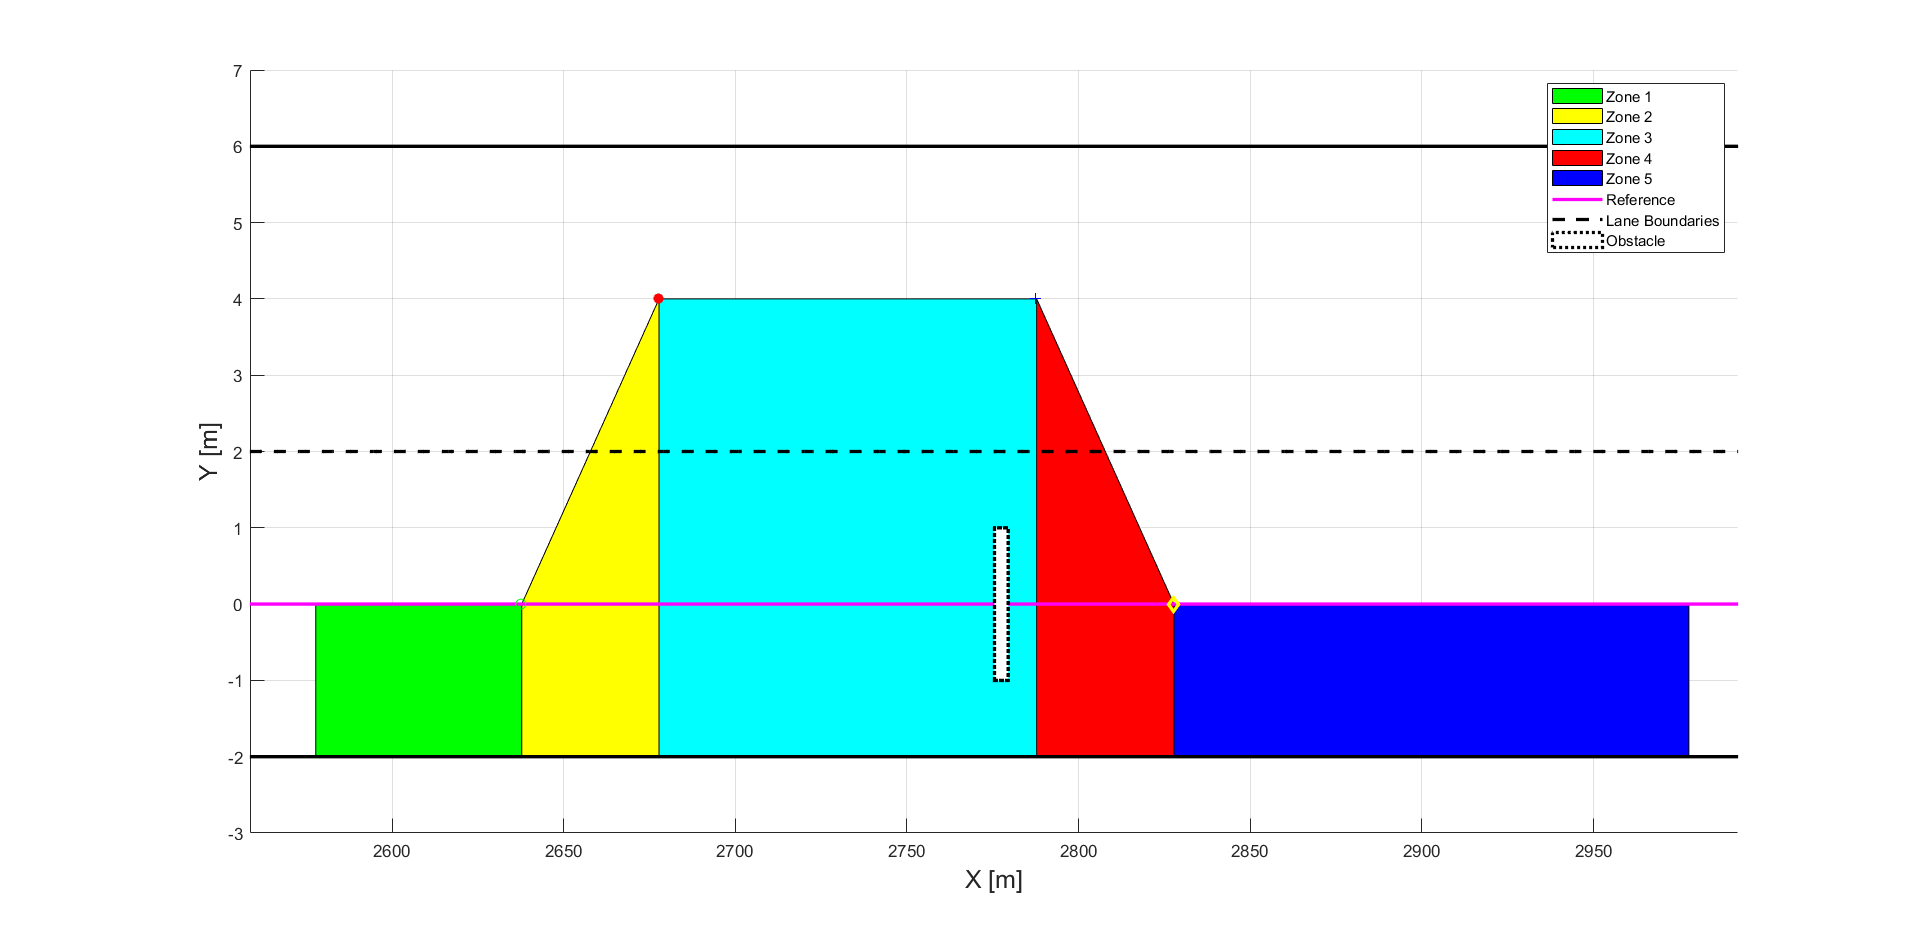
\includegraphics[width=1\textwidth]{Figures/Zones.png}
    \caption{Zones defined for obstacle avoidance}
      \label{fig:Zones}
\end{figure}
In Figure \ref{fig:Zones} the aforementioned zones are depicted on a straight line with a reference speed of 100 km/h. In zones 1 and 5, as previously said, the obstacle is too far from the vehicle to be a problem, so no procedure is applied to the controller.
In zone 2, the yellow one in the figure, the vehicle should pass in the left lane. To do so, we defined two points, represented in the figure with a green $\circ$, which is called the \textit{Detection Point}, and the red circle that is the \textit{Safe Point}. The latter is defined as the projection on the left lane of the point in the reference trajectory at a distance equal to the safety one. To let the controller move on the path defined by these two points, we have exploited the \textit{Custom Constraint} of the MPC block in Simulink.\\
As briefly explained in Section \ref{chap:Controller}, linear combination of inputs and states can be set as constraints for the controller. To accomplish our task, we have defined 2 constraints on the \textit{x} and \textit{y} states, which result in two lines representing an upper and a lower bound for the vehicle position during the overtaking maneuver. Looking at the example in the Figure \ref{fig:Zones}, the lower bound becomes the border of the polygon defined by zones 2, 3 and 4, while the upper bound is the left limit of the road, that is to say the left border of the left lane.\\
For what concerns the lower bound for constraints in zone 2, it is completely defined by the line passing from the two aforementioned points.\\
In zone 3, the vehicle should stay in the left lane. To define constraints in this zone, we have set as lower bound the projection of the reference trajectory on the left lane, instead of the straight line connecting points from the start (red circle) to the end (blue cross), since the former method allows to track both straight and curved paths. One limitation of the \textit{linear} constraints is that they can only define \textit{linear} relation between states, thus when the path is curved, we have to approximate it to a straight line, but this can cause errors because the controller tries to satisfy the constraint for all the timesteps in the prediction horizon, so resulting in a reduced or increased distance with respect to the points in the reference map. To limit this effect, we have inserted a correction factor to the constraint generated.
\begin{figure}[H]
    \centering
    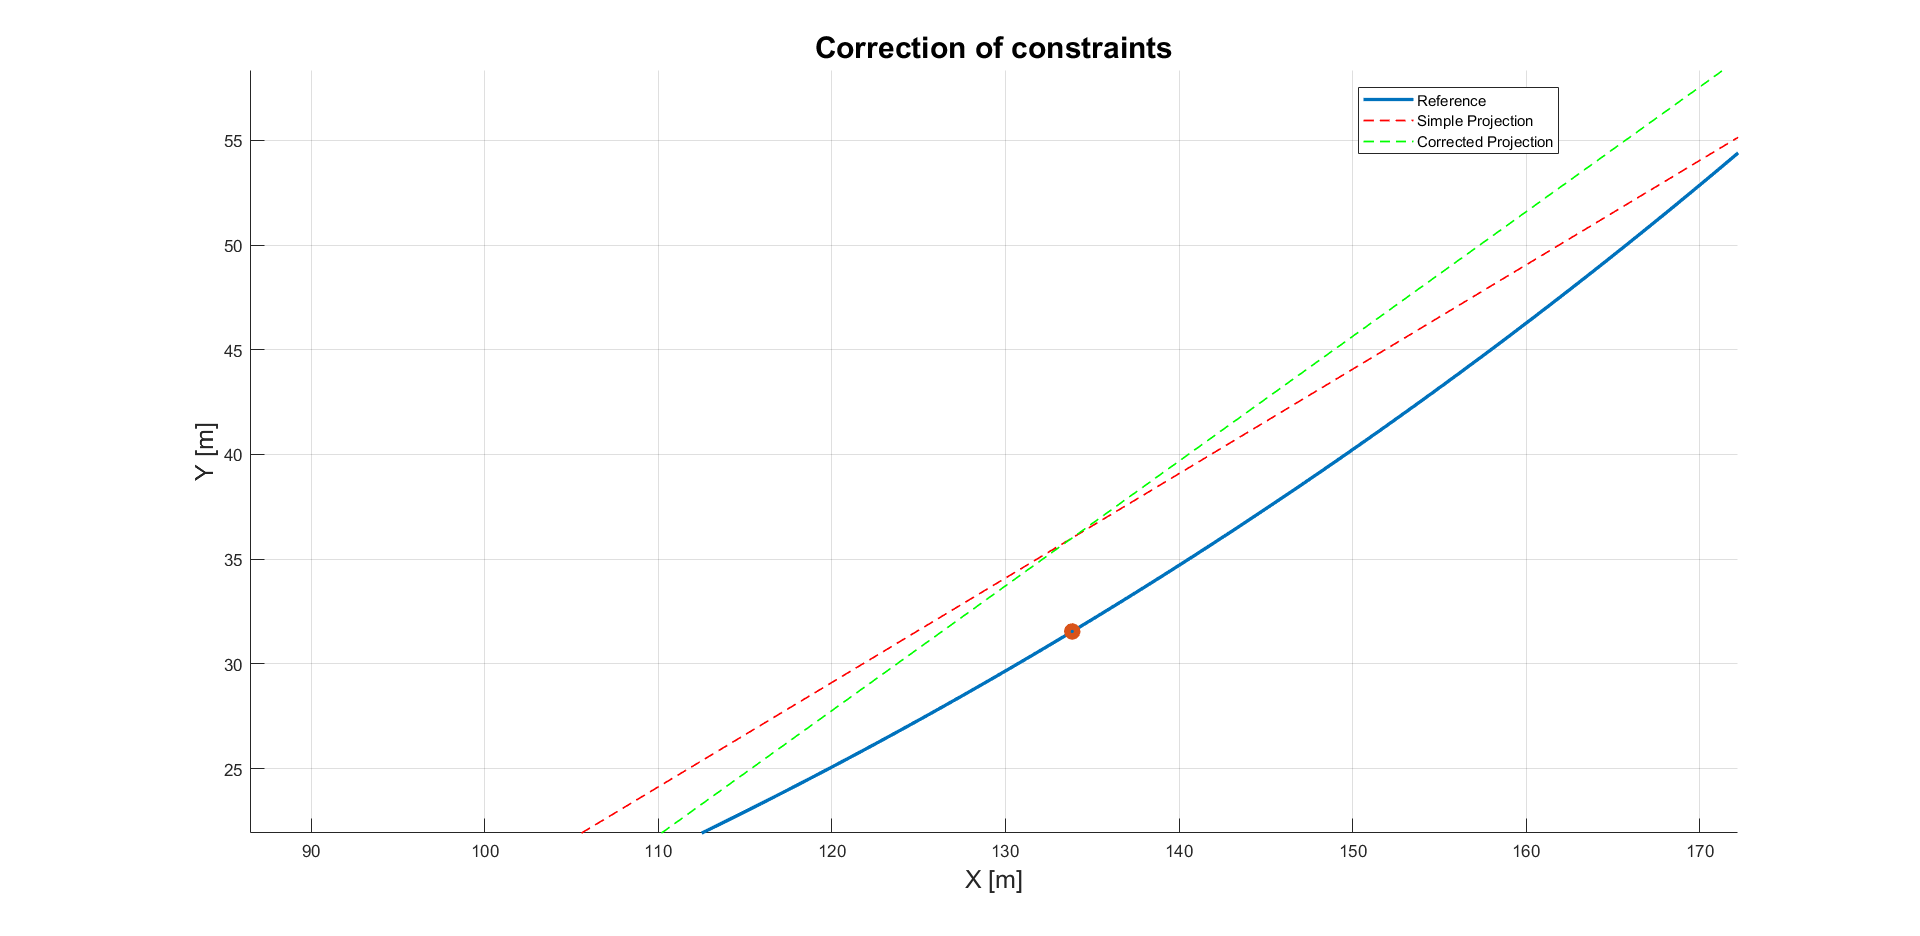
\includegraphics[width=1\textwidth]{Figures/ConstraintCorrection.png}
    \caption{Constraints generated in a curved path with 300 m radius at 50 km/h, with and without the correction factor}
      \label{fig:CorrectionConstraint}
\end{figure}
In figure \ref{fig:CorrectionConstraint} is represented a case where the reference road is a left curve with 300 meters radius. The dashed red line is the projection of the road approximated with the slope of the reference in the point where the controller is called, while the green dashed line is the projection evaluated with the correction factor. As can be seen, the original projection "collapse" on the reference path before the corrected one, resulting in a reduction of the distance from the reference during the predicted horizon and a consequent reduction of distance between the trajectory and starting lane, occupied by the obstacle.\\
This corrected constraint is evaluated according to the following procedure:
\begin{enumerate}
    \item An approximation of the \textit{curvature} of the road is evaluated as the mean value of the reference angle in the prediction horizon: $curvature = \frac{\sum_{i=0}^{p}\theta_i-\theta_0}{p}$;
    \item The correction factor is: $416\cdot\frac{|curvature|}{V}$, where the coefficient 416 has been found empirically by simulations;
    \item The \textit{CorrectedSlope} is given by the road slope ($tan(\theta_r)$) plus the correction factor;
    \item The intercept for the constraint line is given by:\\
    $CorrectedIntercept = y_r + Lw/cos(\theta_r) - CorrectedSlope\times x_r$\\
    where $x_r$, $y_r$, and $\theta_r$ are the reference trajectory values at the first timestep of the prediction horizon, and $Lw$ is the lane width;
    \item The constraint is applied as $y > CorrectedSlope\times x + CorrectedIntercept$.
\end{enumerate}
Obviously, when the reference path is straight, the correction function becomes 0 and the constraint is the simple projection of the road.\\
In zone 4, the situation is analogous to the one in zone 2, with the only difference that here we are \textit{``relaxing"} the constraint, allowing the vehicle to come back to its original position on the right lane. The bound here is defined by the blue cross point, called \textit{End Point} and the yellow diamond point, called \textit{Entry Point}.\\
To define these bounds in a suitable form for the controller, we have to transpose information in a matrix form, describing two line equations:
\begin{equation}
    y > m_{lower}x + q_{lower}
\end{equation}
\begin{equation}
    y < m_{upper}x + q_{upper}
\end{equation}
where $m$ is the slope of the constraint and $q$ is the intercept of the constraint.
Slope of the constraint can be evaluated by calculating the tangent of the road orientation when we are considering the upper bound or the zone 3, while it is evaluated as the slope between the points defined above in zones 2 and 4.\\
The intercept is given by the projection of the reference trajectory, on the left lane center line for zone 3 and on the left road limit for the upper bound, or it is evaluated by inverting the line equation in the changing lane maneuvers.\\
To let our algorithm work on all the quadrants, we make a check of the reference trajectory orientation and we adapt the constraint generation to the case we are in. This check projects the constraints on the $x$ axis rather than $y$ if the road inclination is closer to the vertical line in the X-Y plane, moreover it defines which are the relations between the bounds and the reference trajectory, intended as \textit{``lower than"} or \textit{``greater than"}, according to the direction of the vehicle and its left.
\subsection{Multiple obstacles avoidance}
The procedure described until now shows how the controller sets constraints when an obstacle is detected, but when multiple obstacles are present, things can become harder.\\
If two obstacles are very far one from the other, at least 400 m, they can be treated as single obstacles in sequence, but if they are close, a new definition of the zones is needed. In detail, we decided to control the position of the next obstacle when we reach the \textit{End Point} of the previous. In this case, we can decide whether to come back in the right lane or to stay in the left lane and continue the overtaking maneuver. The procedure follows the rules below:
\begin{itemize}
    \item if the next obstacle is more than 400 m far from the previous one, it is treated as an independent single obstacle;
    \item if the next obstacle is in the range 400 m and 210 m  from the previous obstacle, it is not detected when the vehicle is in the \textit{End Point} of the previous obstacle. Here vehicle simply comes back to the right lane and when the next obstacle is detected, it is treated as a single one;
    \item if the next obstacle is closer than 210 m from the previous one, it is detected when the vehicle is in the \textit{End Point} of the latter, so here a decision is taken:
    \begin{enumerate}
        \item the next \textit{Detection Point} is after the previous \textit{Entry Point} $\xrightarrow{}$ the vehicle reenters in the right lane and starts the new overtaking maneuver when it reaches the next \textit{Detection Point};
        \item the next \textit{Detection Point} is before the previous \textit{Entry Point} $\xrightarrow{}$ the vehicle stays in the left lane and sets as target the next obstacle, so then it repeats this procedure when the next \textit{End Point} is reached.
    \end{enumerate}
\end{itemize}
To implement this control strategy in the simulation environment, we have used a counter on the obstacle, which takes into account if an obstacle has already been passed and in that case the detection algorithm neglects it, considering directly the next obstacle.\\
In reality, of course, a counter is not a feasible solution since it is impossible to know how many obstacles will be detected during a trip, but advanced navigation and sensor systems can detect and classify obstacles, and then can understand whether they have been passed or not, so our assumption is justified.

